\documentclass[compress,11pt]{beamer}
%\includeonly{pendel}
\usetheme{Ilmenau}
%\usetheme{fau-4-3}
%\usecolortheme{beaver}
\beamertemplatenavigationsymbolsempty
\usepackage[ngerman]{babel}
\usepackage{marvosym}
\usepackage{multimedia}
\usepackage[utf8]{inputenc}
\usepackage{amsmath}
\usepackage{amsfonts}
\usepackage{amssymb}
\usepackage{graphicx}
\usepackage{esvect}
%\author{}
\title{EP Gruppe 8}
%\setbeamercovered{transparent}
%\setbeamertemplate{navigation symbols}{}
%\logo{}
%\institute{}
%\date{}
%\subject{}
\usepackage{verbatim}
\begin{document}

\section{Aufgabe 1}
\begin{frame}

\end{frame}


\section{Aufgabe 2}
\begin{frame}Schaltbild des ersten Aufbaus:\\
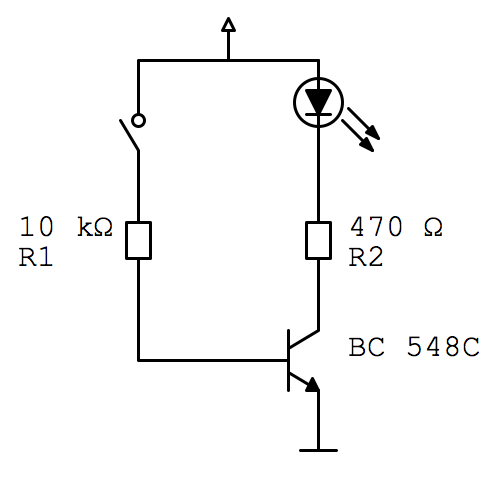
\includegraphics[width=.7\textwidth]{schaltbilder/2}\\
\end{frame}
\begin{frame}

\subsection{Erste Version der Schaltung}
\begin{itemize}
\item Transistor hier als Schalter, da Strom nur fließt, wenn $U_{CE} \neq 0$
\item Sobald der Schalter in der ersten Schaltung geschlossen ist, liegt an Collector und Emitter eine Spannung an und der Transistor lässt durch $\Rightarrow$ Diode leuchtet
\end{itemize}

\end{frame}

\subsection{Zweite Version der Schaltung}
\begin{frame}
Schaltbild des zweiten Aufbaus:\\
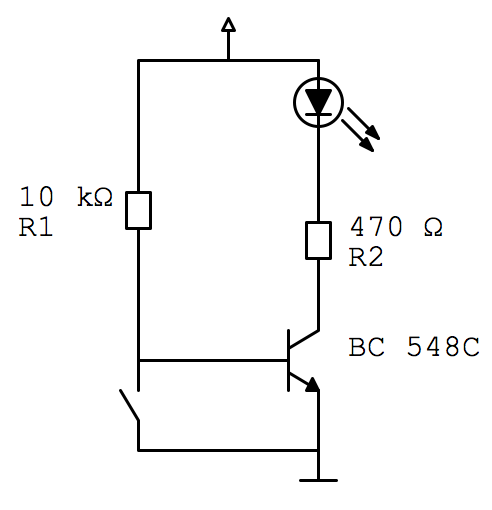
\includegraphics[width=.7\textwidth]{schaltbilder/21}\\

\end{frame}
\begin{frame}
\begin{itemize}
\item Jetzt liegt konstante Spannung an Collektor und Emitter $\Rightarrow$ Transistor sperrt nicht und Diode leuchtet
\item Sobald Schalter geschlossen wird, wird die Basis kurzgeschlossen, also $U_B = 0$ $\Rightarrow$ Transistor sperrt und Diode leuchtet nicht
\end{itemize}
Beide Schaltungen sind aber physikalisch äquivalent
\end{frame}

\begin{frame}

Verwendet wurde eine blaue LED\\
LED sollte nach Aufgabenstellung nur mit einem Strom von max. $20 mA$ betrieben werden\\
Mit "Forward Voltage" $U_F = 3.6 V$ aus dem Datenblatt ergibt sich als Vorwiderstand

\begin{equation}
R_{2,min} = \frac{3.6 V}{20 mA} = 180 \Omega
\end{equation}
Verwendet wurde aber ein $470 \Omega$-Widerstand

\end{frame}
\begin{frame}
Strom durch Basis/Schalter:
\begin{equation}
I_B = \frac{U}{R_1} = \frac{9 V}{10 k\Omega} = 0.0009 A
\end{equation}
Strom durch LED $=$ Strom durch $R_2$:
\begin{equation}
I_C = \frac{U_{R_2}}{R_2} = \frac{6.56 V}{470 \Omega} = 13.957 mA
\end{equation}
\end{frame}
\begin{frame}
Zur Bestimmung der Arbeitspunktes muss $U_{CE}$ noch ermittelt werden:
\begin{equation}
U_{CC} = U_{LED} + U_R + U_{CE} \Rightarrow U_{CE} = U_{CC} - U_{LED} - U_R
\end{equation}
\begin{equation}
= 9 V - 6.56 V -3.6 V = -0.12 V
\end{equation}
$\Rightarrow$ Schwellenwiderstand der LED muss kleiner sein als 3.6 V \\ $\Rightarrow$ $U_{CE}$ aber dennoch klein \\ $\Rightarrow$ Transistor im Sättigungsbereich\\
Transistor als "Schalter", da die CE-Strecke nur leitet, wenn$I_B \neq 0$
\end{frame}








\section{Aufgabe 3}
\subsection{Common-Emitter}
\begin{frame}
Schaltbild:\\
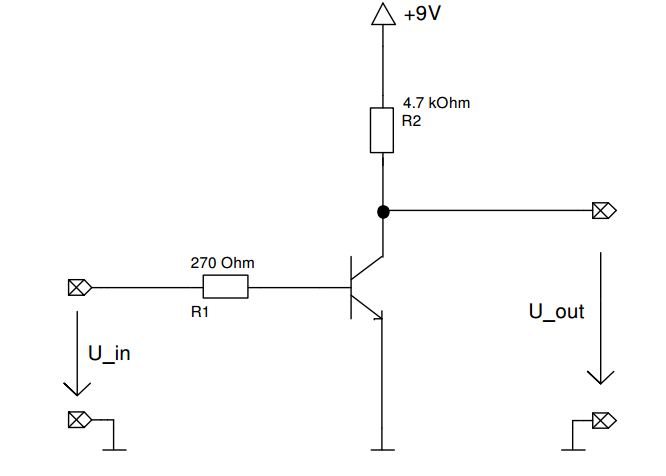
\includegraphics[width=.7\textwidth]{schaltbilder/schalt_3a}\\
Durchfführung:\\ Schaltung wird bei $U_{in}$ mit einer 1kHz-Spannung betrieben, die Amplitude beträgt 1.2 V. Gemessen wird $U_{CE}$
\end{frame}
\begin{frame}
\begin{block}{Funktionsweise der Schaltung}

\begin{itemize}
\item Bei positiver Eingangsspannung $> 0.7 V$ leitet die Basis-Emitter-Strecke des Transistors
\item Je größer die Eingangsspannung, desto größer ist $I_{BE}$ $\Rightarrow$ $U_{CE}$, die abgegriffen wird, wird dementsprechend kleiner $\Rightarrow$ Schaltung invertiert für Positive $U_{in}$
\item Sobald $U_{BE} < 0.7 V$ $\Rightarrow$ Transistor sperrt und Ausgangssignal entspricht den $9 V$ der Gleichspannung
\item Basiswiderstand $R_1$ bestimmt Arbeitspunkt der Schaltung und kann zu dessen Regulierung verwendet werden
\end{itemize}
\end{block}
\end{frame}

\begin{frame}

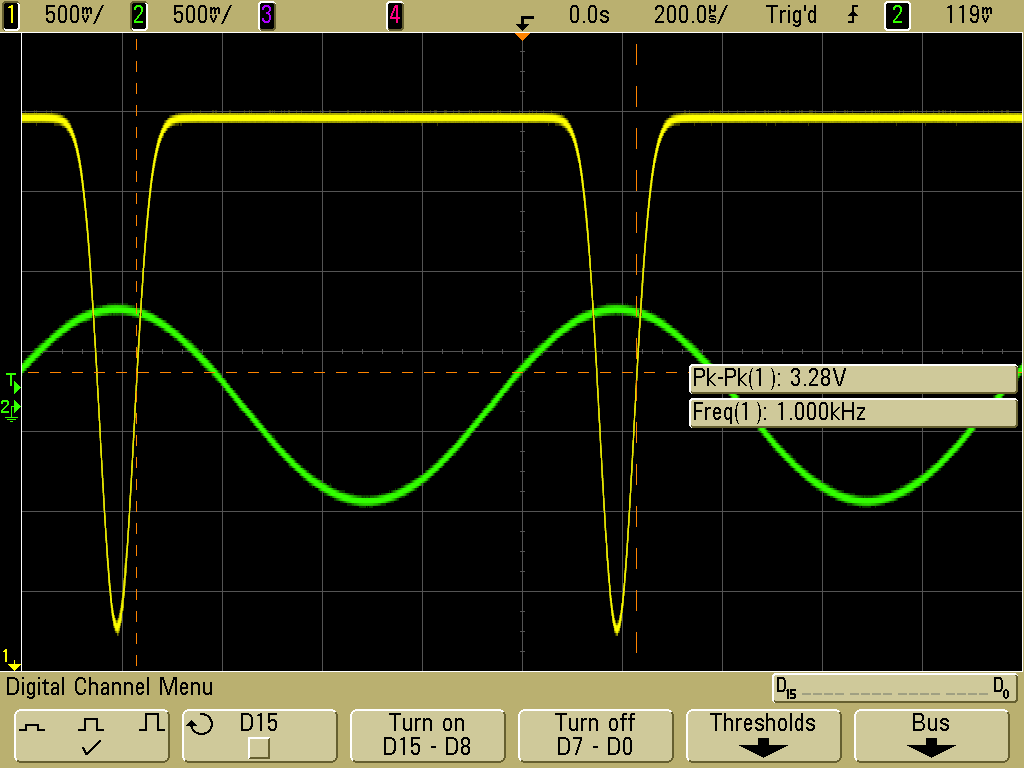
\includegraphics[width=.7\textwidth]{../daten/oszi/scope_45}\\
\begin{block}{Beobachtung:}
Gemessene Amplitude bei Sinusbergen der Eingangsspannung: $U_{out} = 3.28 V$\\
Sonst: $U_{out} = 9 V$
\end{block}
\end{frame}
\begin{frame}
Berechnung der Verstärkung:\\
Nach Vorlesung folgt:
\begin{equation}
U_{out} = U_{cc} - h_{FE} \cdot \frac{R_C}{R_B} \cdot (U_{in} - U_{BE}) \Rightarrow h_{FE} = \frac{(U_{cc} - U_{out})}{(U_{in} - U_{BE}) \cdot \frac{R_C}{R_B}}
\end{equation}
Einsetzen ergibt, da $U_{in,max} = \frac{U_{pp}}{2} = 0.6 V$ und $U_{BE} = 0.7 V$ (Konstante für Dioden) einen negativen, betragsmäßig großen Wert $\Rightarrow$ $U_{BE}$ muss effektiv kleiner sein als $0.7 V$\\
\end{frame}
\begin{frame}

Taktik:
\begin{itemize}
\item projeziere das Intervall, in dem $U_{out} \neq 9 V$ auf das Eingangssignal (nur bei diesen Spannungen ist $U_{in}$ größer als die Durchlassspannung)
\item lese dort die Differenz von maximalen Amplitude zu Funktionswert ab
\end{itemize}


\end{frame}
\begin{frame}
Ablesen ergibt für $\bigtriangleup t_{peak,out} = 200 \mu s$ : $\bigtriangleup U = (U_{in} - U_{BE}) \leq 1 mV$ \\ Für die Verstärkung ergibt sich mit $0.1 V$ also:
\begin{equation}
h_{FE} = \dots 	= 3.28
\end{equation}
Laut Transistor-Datenblatt liegt $h_{FE}$ zwischen 420 und 800\\
Daher Annahme, dass Transistor nicht unter optimalen Bedingungen arbeitet\\
Und für den Gain ergibt sich:
\begin{equation}
G = -h_{FE} \cdot \frac{R_C}{R_B} = 57.2
\end{equation}
\end{frame}
\begin{frame}
\begin{block}{Verhalten unter Erwärmung}
\begin{itemize}
\item Bei Berührung mit dem Finger nur leichter, nicht nennenswerter Anstieg der Amplitude
\item Effektiver ist das Hinhalten eines Lötkolben ($T \approx 150 ^{\circ} C$) in die Nähe des Transistors  $\Rightarrow$ Amplitude steigt auf bis zu $7.3 V$ an
\end{itemize}
Grund: Leitfähigkeit des Halbleiters verstärkt sich bei höheren Temperaturen
\end{block}
\end{frame}
\begin{frame}
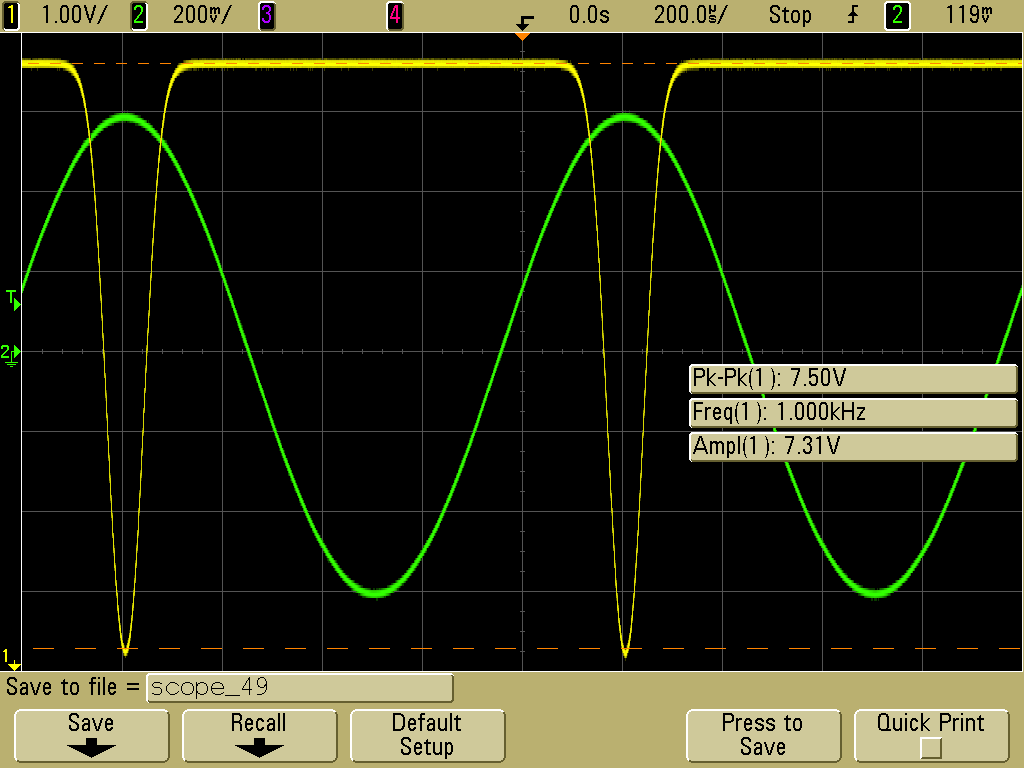
\includegraphics[width=.7\textwidth]{../daten/oszi/scope_49}
\end{frame}
\begin{frame}
Eigenschaften der Schaltung:\\
\begin{itemize}
\item Nicht Linear
\item Spannungen unter $\approx 0.5 V$ werden abgeschnitten $\Rightarrow$ DC-Offset in Spannung nötig, um Signal nur zu verstärken und nicht zu verändern
\item Arbeitspunktbereich im Verstärkungsbereich, wenn Basis öffnet
\end{itemize}
\end{frame}
\subsection{Common-Emitter (verbessert)}
\begin{frame}
Schaltbild:\\
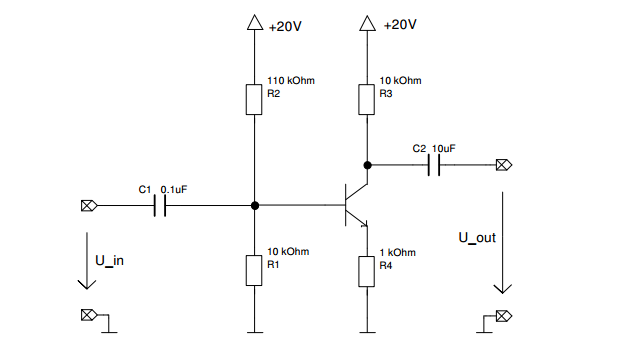
\includegraphics[width=.7\textwidth]{schaltbilder/schalt_3b}\\
Durchführung:\\

Schaltung wurde einmal mit Sinusspannung $U_{in,amp} = 1.25 V$ betrieben, Ausgangssignal wurde invertiert(siehe nächste Folie), aber sonst nicht wesentlich verändert, mit $U_{out,amp} = 11.3 V$ $\Rightarrow$ Amplitudenverstärkung $\approx 9$

\end{frame}
\begin{frame}
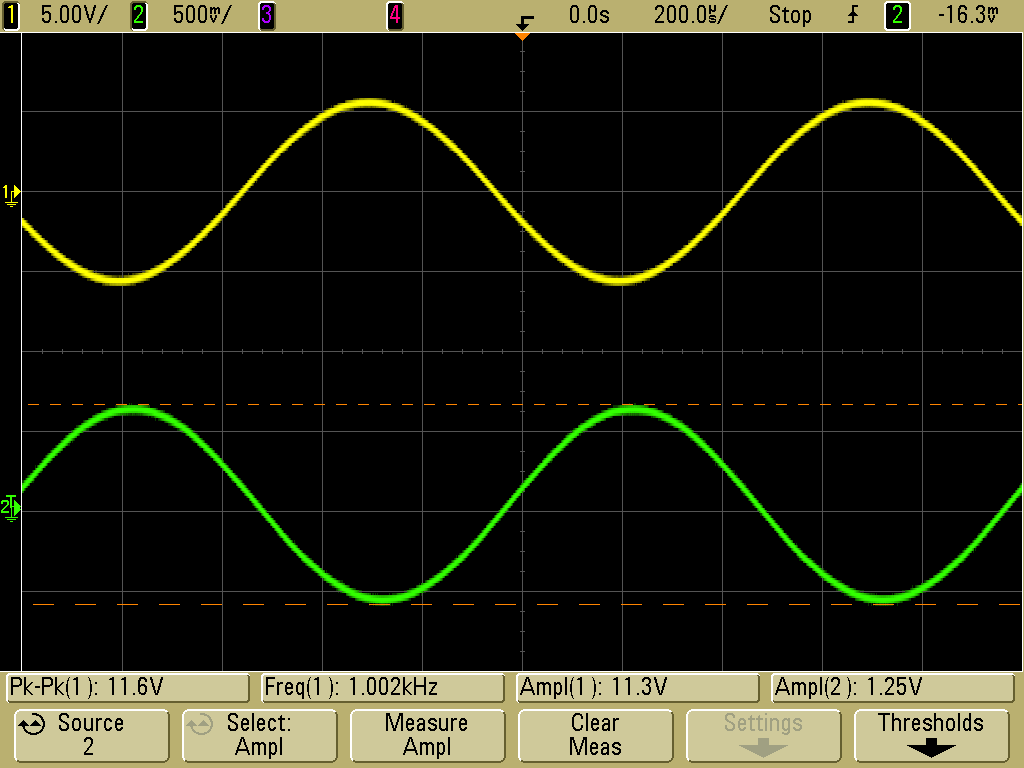
\includegraphics[width=.7\textwidth]{../daten/oszi/scope_51}
\end{frame}
\begin{frame}
\begin{itemize}
\item Arbeitspunkt einer Schaltung ist die Ausgangsspannung, die ohne Eingangssignal gemessen wird
\item Ausgangssignal kann nicht mehr abgeschnitten werden
\end{itemize}
\end{frame}
\begin{frame}
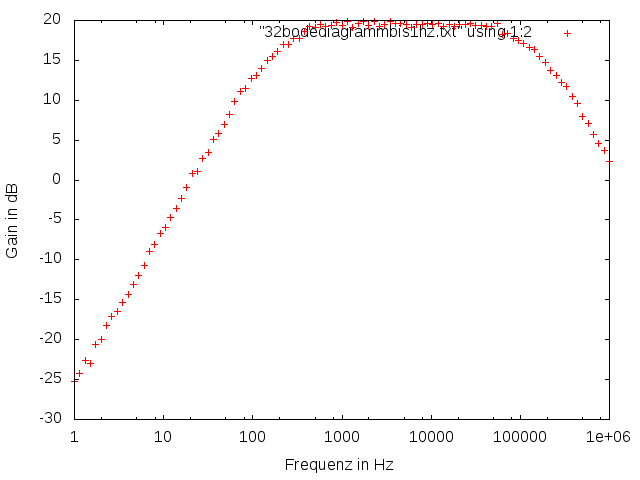
\includegraphics[width=.7\textwidth]{../daten/messungen/3aufgabe/32bodegain}\\
(Gain-)Bodediagramm des verbesserten CE\\
\tiny 
\end{frame}
\begin{frame}

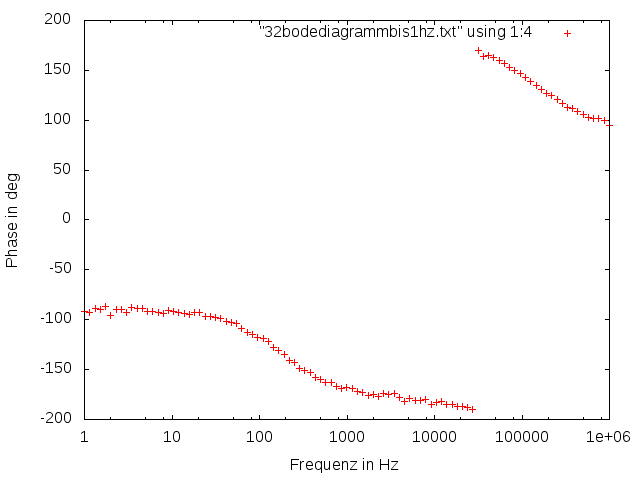
\includegraphics[width=.7\textwidth]{../daten/messungen/3aufgabe/32bodephase}\\
Phasen-Teil des Bode-Diagramms
\end{frame}
\begin{frame}
\begin{itemize}

\item An Ein- und Ausgang des Verstärkers befinden sich Hochpassfilter - daher der Abstieg bei geringen Frequenzen
\item Der Transistor schaltet bei hohen Frequenzen nicht mehr schnell genug (da durch den Spannungsteiler große Widerstände mit der Basis verbunden sind) - daher der Abfall bei hohen Frequenzen

\end{itemize}
Cutoff-Frequenzen (nach Vorlesung):
\begin{equation}
f_{g,in} = (\frac{1}{R_1} + \frac{1}{R_2} + \frac{1}{R_E \cdot (1 + h_{FE})})^{-1} \approx 2523.9 Hz
\end{equation}
\begin{equation}
f_{g,out} = 
\end{equation}
\end{frame}

\subsection{Differenzverstärker}
\begin{frame}
Schaltbild:\\

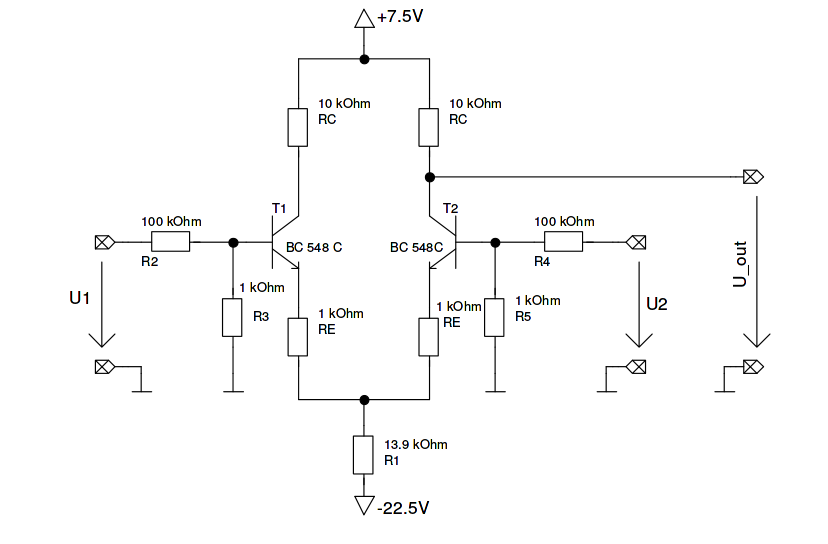
\includegraphics[width=.7\textwidth]{schaltbilder/schalt_3c}\\
Durchführung:\\
Schaltung wurde mit verschiedenen Gleich/Gegentaktspannungen betrieben, die Ausgangsspannungen wurden dann gemessen
\end{frame}
\begin{frame}
\begin{block}{Begriffe}
Gleichtakt: Signale 1 und 2 unterscheiden sich nur um Amplituden
Gegentakt: Signale sind in der Phase versetzt
\end{block}
\end{frame}
\begin{frame}
\begin{block}{Eigenschaften und Funktionsweise der Schaltung}
\begin{itemize}
\item Zwei symmetrisch aufgebaute CE-Schaltungen, über den Emitter-Widerstand verbunden
\item Versorgungs-Strom sowie die einzelnen Eingangsspannungen werden auf beide CE-Schaltungen verteilt
\item Unterschiede der Eingangs-Spannungen führen zu asymetrischen Strömen in der Schaltung, die als $U_{out}$ abgegriffen werden
\end{itemize}
\end{block}
\end{frame}
\begin{frame}
\begin{block}{Theorie}
Gegentaktverstärkung:
\begin{equation}
G_{diff} = \frac{R_C}{2 \cdot R_E} = 5
\end{equation}
Gleichtakt-Verstärkung (sollte nach Vorlesung gleich null sein, zweite Formel aus VL ergibt):
\begin{equation}
G_{CM} = \frac{R_C}{2 \cdot R_1 + R_E} \approx 0.6
\end{equation}
Gleichtaktunterdrückung (nach VL gegen unendlich)
\end{block}
\end{frame}
\begin{frame}
Messung ergibt für Gleichtaktbetrieb:
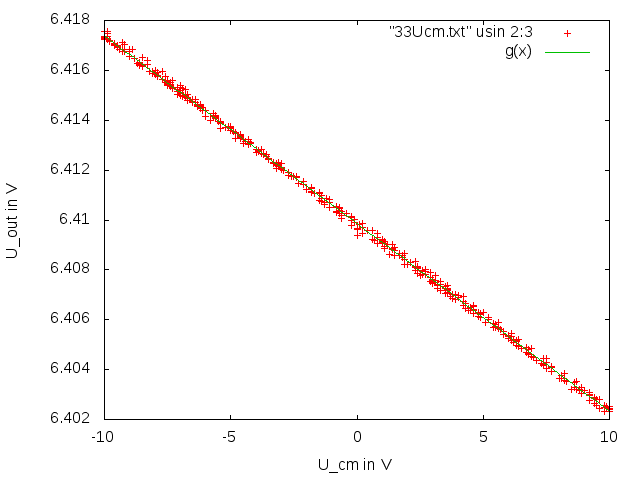
\includegraphics[width=.7\textwidth]{../daten/messungen/3aufgabe/1cm}\\
\end{frame}
\begin{frame}
und für Gegentaktbetrieb:
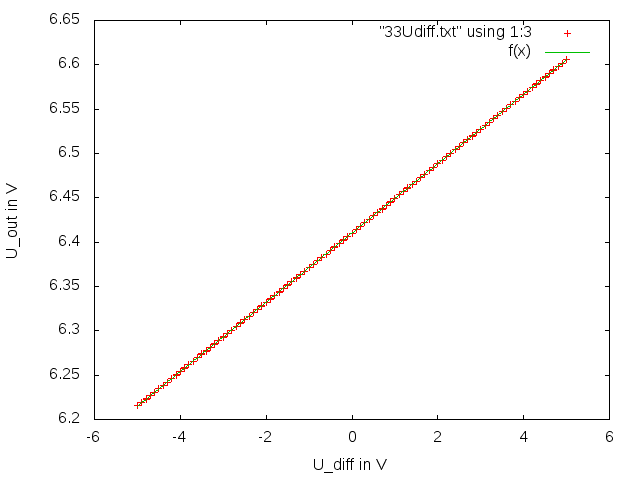
\includegraphics[width=.7\textwidth]{../daten/messungen/3aufgabe/1diff}\\
\end{frame}
\begin{frame}
Werte der Verstärkung $\approx$ Steigung der Regressionsgeraden:

\begin{equation}
G_{CM} = -0.000752511
\end{equation}
\begin{equation}
G_{diff} = 0.0390561
\end{equation}
\begin{equation}
CMRR = |\frac{G_{diff}}{G_{CM}}| = 51.901
\end{equation}

\end{frame}
\begin{frame}
Folgerung:\\
\begin{itemize}
\item Linearer Verlauf (ziemlich genau)
\item Widerstände dämpfen und verursachen Abweichungen
\end{itemize}
Arbeitspunkt ist im Kennlinienfeld durch $I_C$ und $U_{CE}$ bei U1, U2 = o festgelegt, $I_C$ wurde aber nicht gemessen
\end{frame}
\subsection{Differenzverstärker mit Konstantstromquelle}
\begin{frame}
Schaltbild:\\
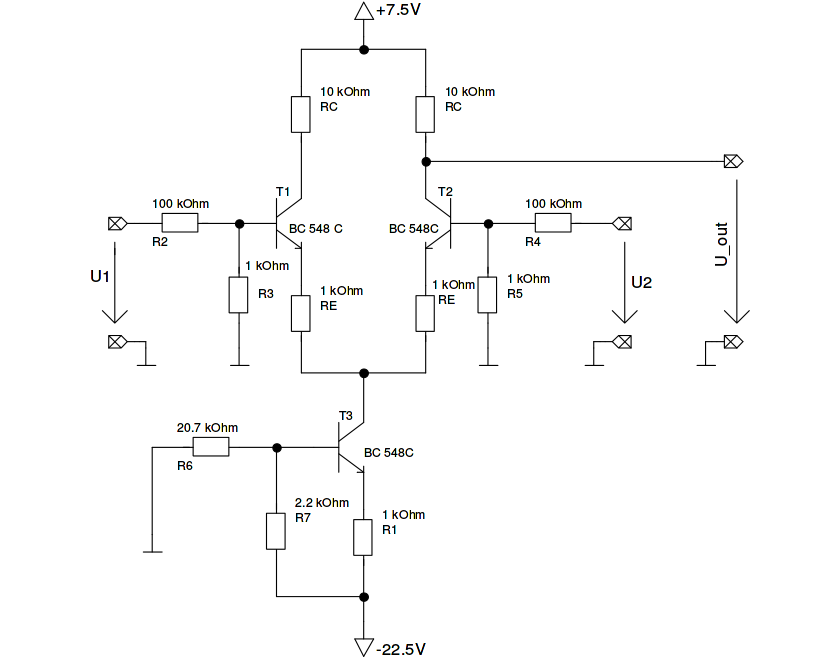
\includegraphics[width=.7\textwidth]{schaltbilder/schalt_3d}\\
Durchführung genau wie bei vorheriger Schaltung
\end{frame}


\begin{frame}
Messung ergibt für Gleichtaktbetrieb:
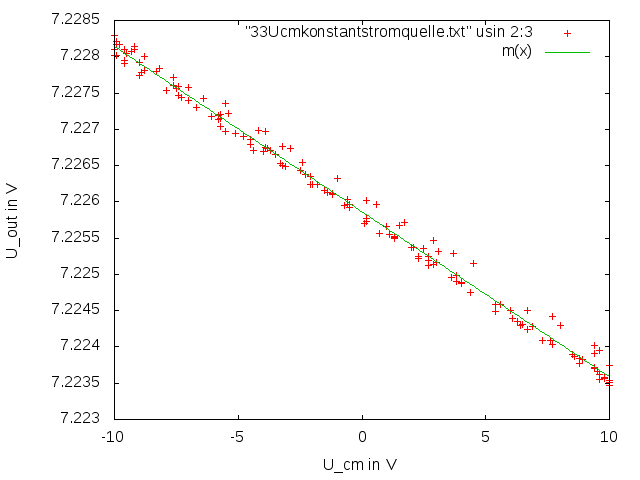
\includegraphics[width=.7\textwidth]{../daten/messungen/3aufgabe/2cm}\\
\end{frame}
\begin{frame}
und für Gegentaktbetrieb:
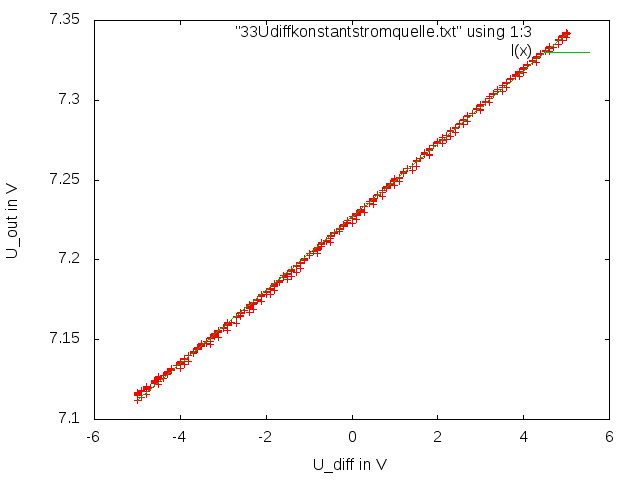
\includegraphics[width=.7\textwidth]{../daten/messungen/3aufgabe/2diff}\\
\end{frame}
\begin{frame}
\begin{equation}
G_{CM} = -0.000227725
\end{equation}
\begin{equation}
G_{diff} = 0.022943
\end{equation}
\begin{equation}
CMRR = |\frac{G_{diff}}{G_{CM}}| = 100.75
\end{equation}
Konstantstromquelle verbessert Gleichtaktverstärkung

\end{frame}
\end{document}
